\documentclass{article}

% if you need to pass options to natbib, use, e.g.:
% \PassOptionsToPackage{numbers, compress}{natbib}
% before loading rl_project.

% to compile a camera-ready version, add the [final] option, e.g.:
 \usepackage[final]{rl_project}

% to avoid loading the natbib package, add option nonatbib:
% \usepackage[nonatbib]{rl_project}

\usepackage[utf8]{inputenc} % allow utf-8 input
\usepackage[T1]{fontenc}    % use 8-bit T1 fonts
\usepackage{hyperref}       % hyperlinks
\usepackage{url}            % simple URL typesetting
\usepackage{booktabs}       % professional-quality tables
\usepackage{amsfonts}       % blackboard math symbols
\usepackage{nicefrac}       % compact symbols for 1/2, etc.
\usepackage{microtype}      % microtypography
\usepackage{graphicx}

\usepackage{amsmath}        % for pseudo code
\usepackage{algorithm}      % make pseudo code easier
\usepackage[noend]{algpseudocode}
\usepackage{float}
\usepackage{subcaption}     % specifying captions
\usepackage{wrapfig}

\captionsetup[figure]{font={bf,small}, labelsep=period}

\graphicspath{ {./} } % Store images ins same folder

% Give your project report an appropriate title!

\title{RL Project}


% The \author macro works with any number of authors. There are two
% commands used to separate the names and addresses of multiple
% authors: \And and \AND.
%
% Using \And between authors leaves it to LaTeX to determine where to
% break the lines. Using \AND forces a line break at that point. So,
% if LaTeX puts 3 of 4 authors names on the first line, and the last
% on the second line, try using \AND instead of \And before the third
% author name.

\author{
  Peter Coates  \\
  Dept of Computer Science\\
  University of Bath\\
  Bath, BA2 7AY \\
  \texttt{pmc52@bath.ac.uk}
\And
  Christopher Burton\\
  Dept of Computer Science\\
  University of Bath \\
  Bath, BA2 7AY\\
  \texttt{cb2516@bath.ac.uk}
\And
  Mirco Carciani\\
  Dept of Computer Science\\
  University of Bath \\
  Bath, BA2 7AY\\
  \texttt{mc2886@bath.ac.uk}
}


\begin{document}

\maketitle

\section{Problem Definition}

% A clear, precise and concise description of your chosen problem, including the states, actions, transition dynamics, and the reward function. You will lose marks for an unclear, incorrect, or incomplete problem definition.
For this assignment, we chose to implement and train 3 different RL agents to play the game of Breakout, a 2D game part of the classic Atari 2600.
In the game of Breakout, a player controls a paddle to bounce a ball against a wall composed by a stack of 6 layers of bricks without letting the ball fall behind the paddle. Each time the ball hits a brick, the brick is destroyed and the score is increasaed by 1,4 or 7 points, depending on the color of the brick which was hit. If the ball falls behind the paddle one life is lost. The game ends when all 5 lives are lost.
Four actions are available at each step $t$, namely, fire, no operation (noop), move left and move right.

The agent has to learn to control the paddle to maximize the  total final reward, meaning hit and destroy as many bricks as possible within the 5 lives available. No points are removed when a life is lost. Although Breakout seems a conceptaully easy problem to solve, its vast state space proves very challening for RL methods. The agent needs to figure out which of the available actions is best to take in each state to maximize the future reward. For the scope of this assignment, we will only consider the single player version. The highest score achievable for one player is 864; this is done by eliminating two screens of bricks worth 432 points per screen.

\section{Background}

%A discussion of reinforcement learning methods that may be effective at solving your chosen problem, their strengths and weaknesses for your chosen problem, and any existing results in the scientific literature (or publicly available online) on your chosen problem or similar problems.

\subsection{DQN}
One category of reinforcement learning methods that can be used to solve the game of Breakout is value-based methods which use function approximation.
These methods aim to learn a function $f: (s,a,\theta) \rightarrow \mathbb{R}$, with $s \in S$,  $a \in A$ and  $\theta \in \mathbb{R}^n$ to estimate the action-value functions for each state and therefore determine the optimal action $a$ to take in state $s$.

Deep Q-Network agent (DQN) introduced by Mnih et al., 2015, was the first value-based RL method to surpass human performances at Breakout making it the first candidate algorithm we decided to implement.
Mnih et al., 2015 show how DQN was able to reach an average score of 401, compared to an average score of 31.8 reached in the same testing conditions by a professional human tester.

DQN introduced both a separate \emph{target network} to estimate the next state maximum action value function and \emph{experience replay memory} to avoid correlated data during training. These introductions allowed DQN to achieve stable learning and converge towards an optimal policy.

\subsection{A2C}

An alternative value-based methods are policy gradient methods. Policy gradient methods do not need to consult a value function and, instead, learn a parameterised policy to select actions (Sutton and Barto, 2018). In selecting actions using a parameterised policy, policy gradient methods use \emph{action preferences} rather than action values. This distinction is crucial as it confers several benefits to policy gradient methods such as the ability to learn a stochastic optimal policy and have the policy approach a deterministic policy (Sutton and Barto, 2018).

A Policy-Gradient method that has been shown to be effective on similar tasks to Breakout is Actor-Critic. An asynchronous, extended version of Actor Critic called Asynchronous Advantage Actor-Critic (A3C) was implemented by Minh et al (2016) to mitigate issues with instability due to temporally correlated data across time-steps (Li, Bing and Yang, 2018). The Advantage component of A3C refers to the use of an advantage function in the reinforcing signals sent to the actor. This advantage value quantifies how much better or worse an action is than the average available action by using the critic's valuation of states (Graesser and Loon, 2020). A synchronous version of A3C that implements the advantage function but does not execute multiple agents in parallel is known as Advantage Actor Critic (A2C). Whilst both methods provide strong results on Breakout and similar tasks, results from Wu et al. (2017) indicate that A2C is a more suitable algorithm for the problem of Breakout than A3C.

\subsection{Async Q-Learning}

Mnih et al (2016) presented asynchronous variants of Q-Learning.
The paper claims the asynchronous variant can produce excellent results on single multi-core CPUs with training times of just a few hours. The results published by Mnih et al (2016) are impressive and show that after 10 hours training with Breakout, Async Q-Learning scored 240, whilst DQN only managed 25.

Unlike DQN, the asynchronous methods do not require a replay memory buffer as multiple agents working in parallel means that the data is fragmented and sufficiently decorellated.

\section{Method}
%A description of the method(s) used to solve your chosen problem, an explanation of how these methods work (in your own words), and an explanation of why you chose these specific methods.
\subsection{DQN}

DQN was derived from Q-Learning where the action-value function is estimated by a nonlinear function, more precisely, by a deep neural network.

\begin{equation}
Q(S,A) = f(S,A,\theta) = \hat{Q}(S,A,\theta)
\end{equation}

Bootstrapping is used to update the action value function as shown in the equation below.
\begin{equation}
\hat{Q}(S,A,\theta) = \hat{Q}(S,A,\theta) + \alpha * \left( r + \gamma \max_{a} \hat{Q}(S',a,\theta) - \hat{Q}(S,A,\theta) \right)
\end{equation}
Where $\alpha$ is the learning rate and $\gamma$ is the discounting factor for future rewards.

The function parameters are updated in the direction that minimizes the loss between the current action value function estimation and its update. The weight update is achieved by a single step of gradient descent as described in equation \ref{eqn:weightupdate}.

\begin{equation}
\label{eqn:weightupdate}
\theta_{t+1} = \theta_{t} + \alpha \left( r + \gamma \max_{a} \hat{Q}(S',a,\theta_{t}) - \hat{Q}(S,A,\theta_{t}) \right) \nabla_{\theta_{t}} \hat{Q}(S,A,\theta_{t})
\end{equation}

As a result of the weights update at each step $t$, the action-value function estimation $\hat{Q}(S, A,\theta_{t})$ is updated towards a moving target as the next state maximum action value function $\max_{a} \hat{Q}(S',a,\theta_{t})$ will also change. One of the major breakthroughs introduced by Mnih et al., 2015 was the introduction of separate networks. One network (q-value network), is used to estimate the action value functions of the current state $S$, while a separate network (target network) is used to estimate the action value functions of the next state $S'$. The weights of the target network are kept constant for a number of iterations before being synched with the q-value network weights. By using a constant target network, the q-value network can be updated towards a stable target limiting instability during training.

DQN also uses a replay memory buffer to store the last $N$ interactions with the environment. At each step, the following details are recorded in the memory: state $S$, action $A$, reward $R$, observed next state $S^\prime$ and flag indicating whether or not $S^\prime$ is terminal.

A subset $n \in N$ of experiences is then selected and used to update the q-value network weights using equations \ref{eqn:weightupdate}. This allows the agent to train on time uncorrelated data.

Our DQN implementation tests three different methods to retrieve the experiences from the experience replay buffer.
\begin{enumerate}
  \item Uses the implementation of Mnih et al., 2015 where the $n$ experiences are selected at random from the buffer of capacity $N$.
  \item Selects half randomly and half using cosine similarity to select experiences that closely matching the next state $S'$.
  \item Uses cosine similarity to select experiences that closely matching the next state $S'$.
\end{enumerate}
The idea behind the cosine similarity approach is to create a synthetic dejavu.

DQN uses an $\epsilon-greedy$ policy to provide exploration whilst choosing the best action $A*$ from all available actions in the next states.
The exploration factor $\epsilon$ is reduced from an initial value of 1 to 0.1 over 1M steps and kept constant thereafter.

The loss function used to calculate the weight updates is the Huber loss which improve stability by clipping the gradient of the loss with respect the estimated action value function. Mnih et al., 2015 shows how this improves stability during training.

Two identical convolutional neural networks (CNN) are used as function approximations for the Q values. The raw pixel data output by  whilst playing Breakout is preprocessed before being used as input to the CNNs for state $S$. The output of the CNNs are the Q values for each action available in that state $S$.
The preprocessing crops the raw data, resizes to 84x84 pixel and converts to grey scale. And, to give the CNN the information about the ball trajectory, the state $S$ is a stack of the current and 3 previous frames.
DQN pseudo-code is shown in \nameref{dqn_pseudo}

\subsection{A2C}

The second method chosen to solve our specific problem of Atari Breakout is Advantage Actor-Critic (A2C). In this implementation, the actor policy is parameterised by a CNN where the parameters are the weights of the neural network. The critic is also implemented as a CNN, with both architectures following a modified version of that used in Minh et al. (2015). For the Actor, the output layer uses a softmax activation function for the output layer with a single neuron for each possible action that the actor can take. This is to achieve a policy parameterisation known as softmax in action preferences (Sutton and Barto, 2018). The critic network uses the same architecture but has a single output neuron with linear activation, representing the action-value that the critic prescribes to a given state. RandomUniform initialisation is used with a small range of min and max values (0 - 0.02) as initial runs of the algorithm showed high sensitivity to initial weights on the output layers, particularly on the actor.

The input to both networks is similar to that used for DQN, and, is implemented using an OpenAIGym provided Atari wrapper that follows the guidelines in Machado et al. (2018). The current and the 3 previous frames are stacked to give the agent context such as the direction the ball is travelling in.

The critic uses a TD update. At each step, the critic network calculates a value estimate for both the previous state and the next-state that the agent is in. The critic uses a bootstrapped estimate of the next state, the reward at $t+1$ and the discount factor to calculate a target value for the state. The mean squared difference between the critic's initial value of the state and the target value is used to update the critic and adjust its estimate of the state closer to the target value. The target TD value is used also to calculate the advantage function for the actor loss by subtracting the critic's valuation of the previous state from the target TD update. The full A2C actor update rule from Yoon (2019) is given below:

\begin{equation}
\nabla_{\theta} J(\theta) = \sum_{t=0}^{T-1}\nabla_{\theta}\log{\pi_{\theta}}(a_{t} | s_{t}) A(s_{t}, a_{t})
\end{equation}
Where:
\begin{equation}
A(s_{t}, a_{t}) = Q_{w}(s_{t}, a_{t}) - V_{v}(s_{t}) = r_{t+1} + \gamma V_{v}(s_{t+1}) - V_{v}(s_{t})
\end{equation}

The first component of the actor loss function is the gradient in parameter space (delta). This value represents the action taken and whether it followed or went against the current actor policy. The delta term implementation in this assignment follows an extended version of the method followed by Wang (2021). The advantage component, which represents the reinforcement signal from the critic, tells the actor whether the action taken was better than the average reward for that state (Positive advantage) or worse (Negative advantage). By multiplying the gradient of action selection with respect to the current policy and a positive or negative advantage value, the actor evaluates the action taken and current policy against the valuation states from the critic. The agent is encouraged to reinforce the current policy if the action taken follows the current policy and the action taken resulted in a value better than the average value for that state or the action taken went against policy which resulted in a lower than average value. Conversely, the agent is encouraged to update away from the current policy if the action followed the current policy and resulted in a worse value than average for the state or if the agent went against current policy and the resulting value was better than the average for the state. Since log probabilities do not tend to 0 when multiplied, they provide better numerical stability during training.

Initial runs showed that even with very small learning rates (1e-5 and below), the agent would find a local minima, selecting the same action every time. Thus, an entropy term has been added to improve training stability. The entropy term, originally proposed by William and Peng (1991) for use with the REINFORCE algorithm, encourages the actor to output a distribution with higher entropy (More even probabilities) by penalising low entropy outputs through the loss function. For example, in an environment with four actions such as Breakout, a maximum entropy output distribution would have a 0.25 probability of selecting each action. The inclusion of the entropy term yields a new update equation below where  $\beta$ is the entropy weight, which is a hyperparameter that controls how much the actor loss comprises of the entropy value.

\begin{equation}
\nabla_{\theta} J(\theta) = \sum_{t=0}^{T-1}-\nabla_{\theta}\log{\pi_{\theta}}(a_{t} | s_{t}) A(s_{t}, a_{t}) + \beta H_{t}
\end{equation}

\subsection{Async Q-Learning}

The third method chosen to solve our specific problem of Atari Breakout is Asynchronous Q-Learning.

Like DQN, Async Q-Learning uses a value network to select actions to take and then uses a target network to estimate an action value that is used to calculate the loss. The weights in the target network are occasionally reset to match the value network.

Where Async Q-Learning differs from DQN is that it runs multiple worker agents in separate processes which share the value and target networks.

Each worker agent uses local copies of the value and target networks to calculate the losses and gradients, then applies them to the  shared networks every few steps as a single batch.
Once the worker agent has updated the shared network, it refreshes the weights in its local copies to match shared ones.

As the updates are done in batches, it is easy to also implement the n-step variant of Async Q-Learning, which according to Mnih et al (2016) offers further performance improvements. (\nameref{async_q_n_step_pseudo})

Having multiple worker agents means that different areas of the game will be explored at the same time.
The different worker agents were given different epsilon values for their $\epsilon$-greedy policies to increase the variety of exploration.
Some experimentation was also done using both decaying epsilon values, and learning rates. However, the time taken to run tests prevented a thorough examination.

A controller process handles the creation of, and communication with, multiple workers and a stats collector.
Each worker plays games of Breakout letting the controller know the results.
The controller keeps track of the total number of episodes completed by all the workers, and uses the stats collector to provide a measure of how well the training is going.

\section{Results}
%result comparison between the 3 approaches.
%how quickly each agent learns
%how well do they perform is absolute terms
%how do they compare  with respect to a human player

Both v4 and v5 of the Arcade Learning Environment (ALE) were used during testing. 

v5 introduces a \emph{repeat\_action\_probability=0.25} meaning that 25\% of the time the action sent by the agent to the Breakout game is ignored, and the previous action is used instead. This makes the environment stochastic and harder to train an agent against. The following results were obtained by training DQN against v5, A2C against v4, and Asynch n-step Q-Learning against both.


\subsection{DQN}
%% Explain the differete experiements
%% PLot the graphs evaluation vs

Different DQN agents with different configurations of memory capacity and experience replay selection were initially tested for 7 million Frames to attest the best hyper-parameter set. The picture below shows the test score trajectories of 4 different DQN agent configurations.
\begin{figure}[H]
\centering
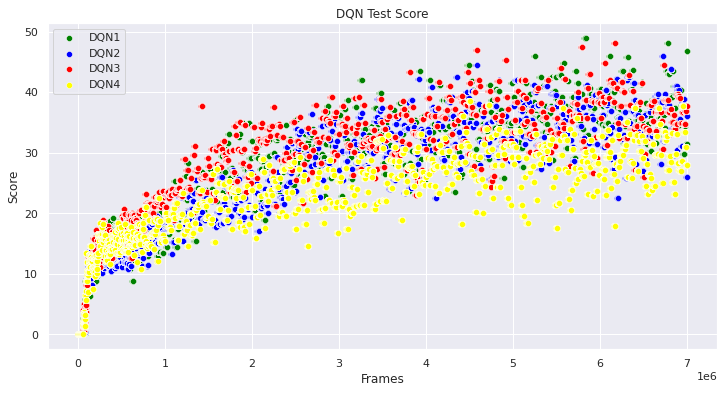
\includegraphics[scale=0.5]{DQNAgentComparison.PNG}
\caption{DQN agent performances comparison over 7M frames. DQN1: N=200k, random experience replay selection. DQN2: N=1M, random experience replay selection. DQN3: N=200k, half prioritized experience replay selection. DQN4: N=500k, full prioritized experience replay selection.}
\label{fig:DQNAgentComparison}
\end{figure}

Due to the amount of time required to train multiple agents, the training process was then resumed up to 24M frames with DQN2 agent only. There was no clearcut winner from the initial test, so DQN2 was chosen because its hyper-parameters mimic the values used by Mnih et al., 2015 which gives a clear baseline for performance comparison.

\begin{figure}[H]
\centering
\begin{subfigure}{0.49\textwidth}
\centering
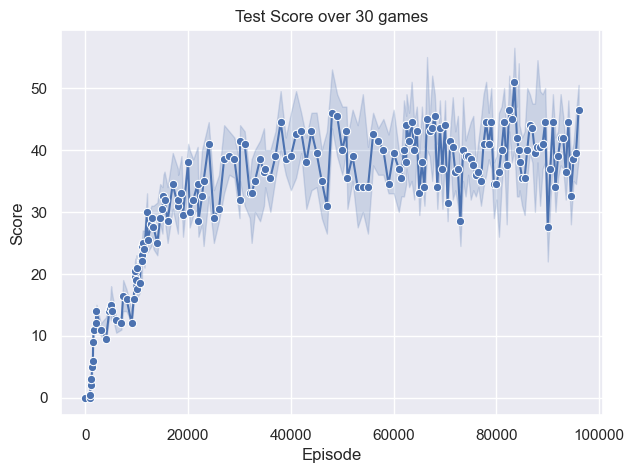
\includegraphics[scale=0.39]{DQNTestScore.PNG}
\captionof{figure}{Test score over 30 games with epsilon = 0}
\end{subfigure}
\begin{subfigure}{0.49\textwidth}
\centering
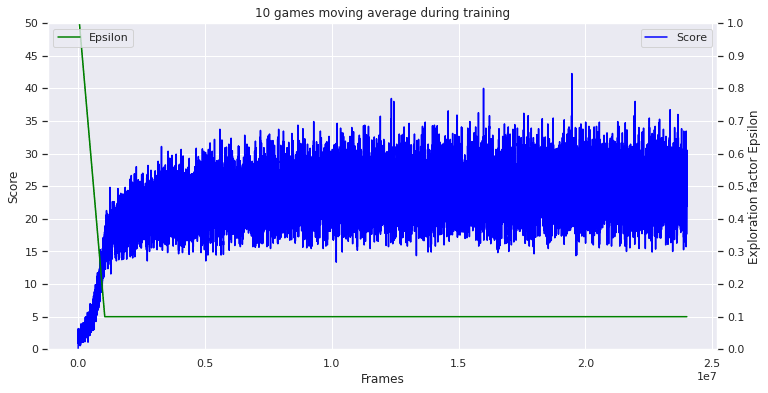
\includegraphics[scale=0.39]{DQNMovAvgTraining.PNG}
\captionof{figure}{10 games score moving average during training}
\end{subfigure}
\caption{DQN2 performances}
\label{fig:DQN2}
\end{figure}


\subsection{A2C}

From episode 1000, the agent shows steady and notable improvement, maintaining a running average of over 10 points by episode 2500.

\begin{wrapfigure}{r}{0.55\textwidth}
\centering
\captionsetup{width=.8\linewidth}
\vspace*{-1cm}
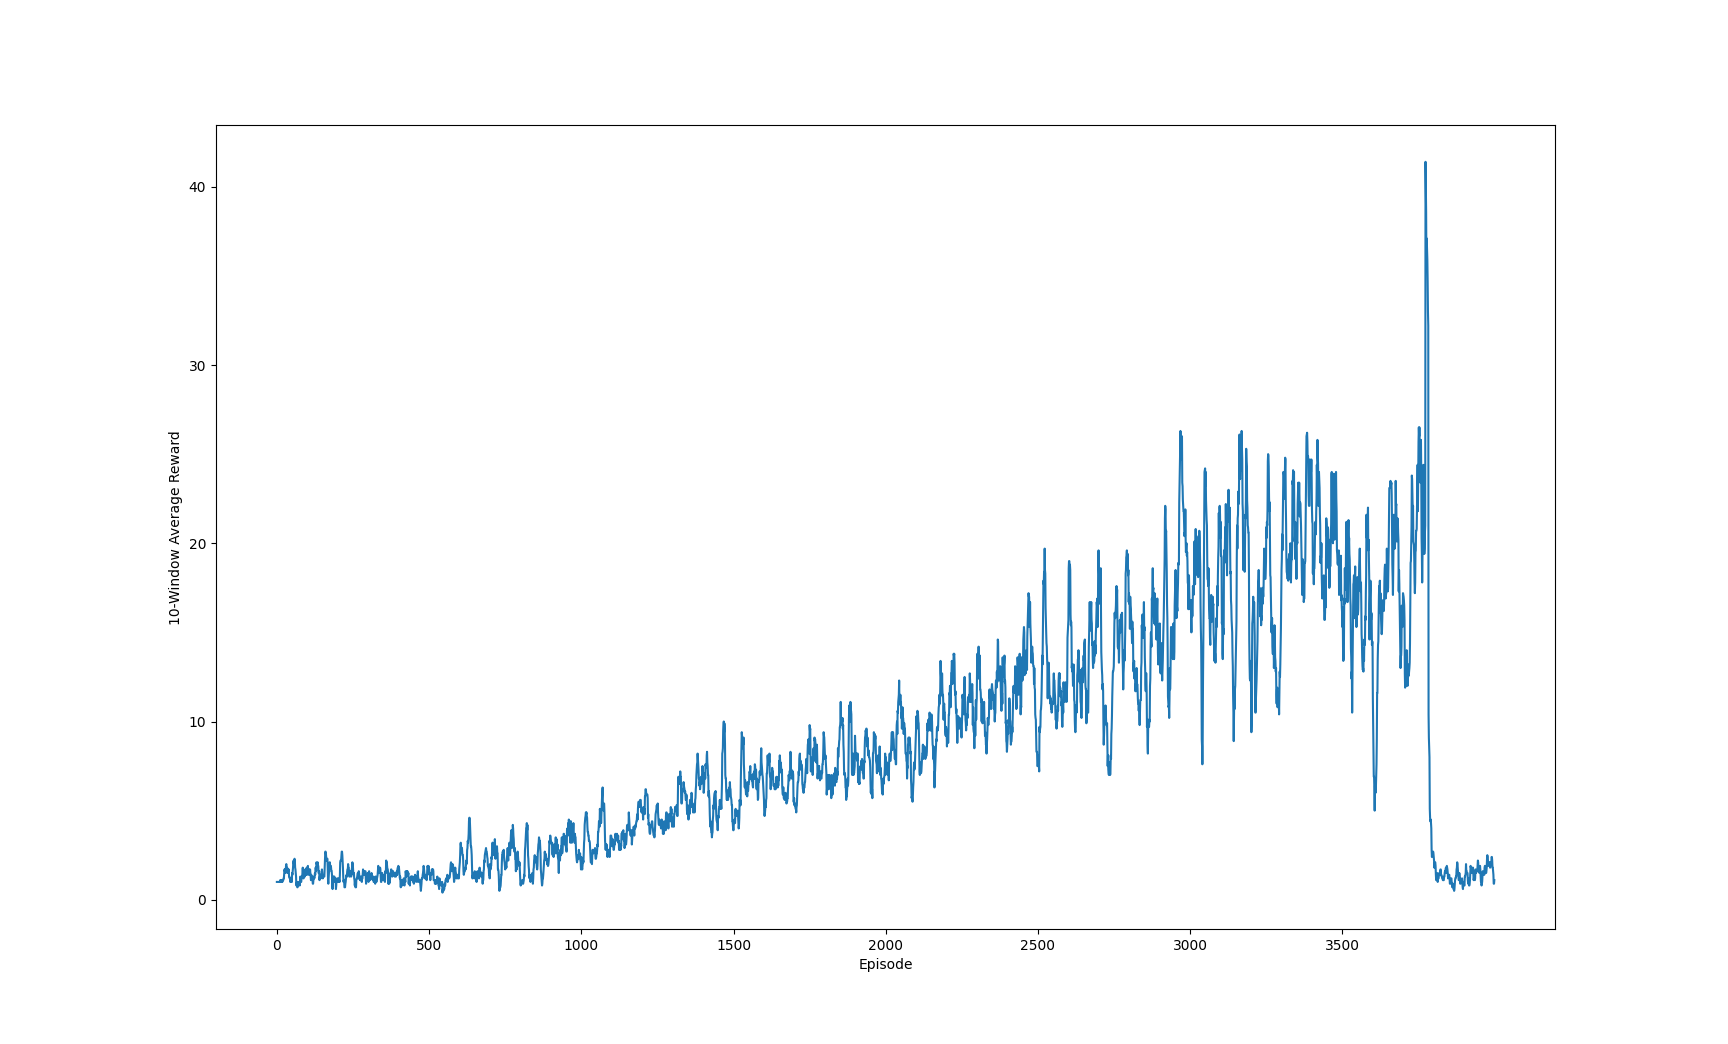
\includegraphics[width=.98\linewidth]{A2C4000.png}
\caption{10-episode running average for Breakout A2C agent over 4000 episodes}
\end{wrapfigure}


 The agent performance peaks around episode 3750 with a 10 game average of 41.4 and peak single game performance of 233.

 Beyond this point the agent shows evidence of overtraining. Performance significantly deteriorates to the level seen in the earliest episodes.

 Observing the actor's softmax output, we see that the agent is outputting almost the same probabilities for every state with very little change in the distribution between states or between episodes.

\subsection{Async Q-Learning}

The figures below show the results from a long run of approximately 40 hours (24 million frames) using Async n-step Q-Learning (n=8). A learning rate of 0.0001, epsilon values in the $\epsilon$-greedy policies varied in different processes and were reduced from a maximum of 0.4 down to 0.1 after approximately a million frames.

\begin{figure}[H]
\centering
\begin{subfigure}{0.49\textwidth}
\centering
\includegraphics[scale=0.4]{"n_step v4 by steps"}
\captionof{figure}{Run against ALE v4}
\end{subfigure}
\begin{subfigure}{0.49\textwidth}
\centering
\includegraphics[scale=0.4]{"n_step v5 by steps"}
\captionof{figure}{Run against ALE v5}
\end{subfigure}
\caption{Long runs of Async n-step Q-Learning against v4 and v5 of the ALE}
\label{fig:ASYNC1}
\end{figure}

The figures clearly show that v5 of the ALE with \emph{repeat\_action\_probability=0.25} is harder to train against than v4 of the ALE which does not have repeat action. Scores achieved with v5 tended to improve at about half of the rate of scores achieved with v4.


\section{Discussion}
    
%An evaluation of how well you solved your chosen problem.

\subsection{DQN}
Mnih et al., 2015 report a maximum average score of 401 after 50M frames. We were not able to replicate the same level of performance. The best average score recorded in our implementation of DQN is 51 at around 21M frames (83500-th episode) Although we could not match Mnih et al., 2015 results, our agent reaches 160\% of human performance.
\begin{table}[H]
\centering
\begin{tabular}{|c | c | c |} 
 \hline
 Human (Baseline) & DQN Implementation & Mnih et al (2015) DQN (50M frames) \\ [0.5ex] 
 \hline
 31.8 & 51 & 401  \\ 
 \hline
\end{tabular}
\end{table}
It was interesting to notice the early difference in performances amongst DQN agents having different memory buffer sizes and experience replay selection methods shown in Figure\ref{fig:DQNAgentComparison}. DQN1 and DQN2 differ in the size of the memory buffer (200K vs 1M), but, no appreciable difference was seen between the two. Comparable results were obtained selecting half of the training samples using cosine similarity. An overall degradation in performances was recorded while only selecting experiences which resemble the agent observed state $S'$. This might suggest that by only selecting experiences which are similar to the current observation a form of data correlation is introduced.

\subsection{A2C}

\begin{table}[H]
\centering
\begin{tabular}{|c | c | c |} 
 \hline
 Human (Baseline) & A2C Implementation & Wu et al. (2017) A2C (50M frames) \\ [0.5ex]
 \hline
 31.8 & 41.4 & 581.6  \\ 
 \hline
\end{tabular}
\end{table}

The A2C implementation was able to significantly outperform a professional human game tester, reaching 130.19\% of human performance. This was achieved in 3,750 episodes (8 hours) of training. The implementation outperforms the human baseline, so, the agent has solved the chosen problem relatively well. Wu et al. (2017) required 14,464 episodes to surpass human performance, whereas our A2C implementation only required 3,774. This shows that our implementation learns quickly.

However, the implementation does not come close to achieving the 100 game running average of 581.6 achieved by the A2C implementation in Wu et al. (2017). The agent training becomes unstable significantly before the timesteps taken in Wu et al. (2017). Interestingly, across several runs, the instability and subsequent local minima appear after a particularly high score (In this case 233), indicating that a potential cause is a very large update to the networks that the agent is unable to properly incorporate. This suggests that a potential route to match the high scores reached in the literature is to reduce the learning rate and training the agent for significantly longer or implementing reward clipping.


\subsection{Async Q-Learning}

The performance of Async n-step Q-Learning and DQN was similar with both achieving an average score around 50 after processing 24 million frames with v5 of the ALE.

Comparing the results from Async n-step Q-Learning and A2C when trained against v4 of the ALE shows that the configuration used for A2C  learns more quickly. Async n-step Q-Learning was slower, but kept on increasing, managing an average score of over 100 after processing 24 million frames.

The results obtained from running Async n-step Q-Learning did not match the results and time scales achieved by Mnih et al (2016). However, they completed approx 25 epochs in 10 hours to get scores in excess of 250. A single epoch being 4 million frames giving 100 million frames in 10 hours. In contrast our implementation is 16 times slower, processing about 6 million frames in 10 hours.

Our results compare favourably with those from Mnih et al (2016). We reached a score of 50 in half the number of frames. However, we have not trained over enough frames to compare final scores.

\section{Future Work}

\subsection{DQN}
Experience replay is a key ingredient in the success of DQN agent. In this assignment random experience replay was implemented, and, although effective, Schaul et al., 2016 work prove that rank-based and proportional based prioritized experience replay improves the agent performances. Narasimhan et al., 2015 also suggest an alternative method of resampling the experiences. The method separates experience into two buckets, one for positive and one for negative rewards. The experiences are then picked from the two buckets by a fixed ratio.

\subsection{A2C}

In the A2C implementation used, the advantage function is calculated using n-step (Where n=1) returns. This only includes one step of actual rewards. Since rewards are generated from a single trajectory, they tend to have high variance but are unbiased. However, the state valuation reflects all trajectories seen so far and thus has lower variance but introduces bias. As a result, the value of n controls the bias-variance tradeoff (Graesser and Loon, 2020).Thus, using 1 step returns provides us with a tradeoff of low variance but introduces significant bias through the reliance on state value.

In contrast, Generalised Advantage Estimate (GAE) overcomes the need to set n as a hyperparameter by using an exponentially-weighted average of advantages calculated with different values of n (Schulman et al., 2015). GAE provides a method by which the low-variance, high-bias one step advantage is most heavily weighted but the lower-weighted contributions from higher values of n still contribute. By tweaking the decay rate of contribution from these higher-variance estimators with higher values of n, GAE allows a more finely controlled tradeoff between bias and variance than the hard cut-off tradeoff in n-step methods (Graesser and Loon, 2020). In comparison to the 1-step method implemented, this is likely to allow a significant reduction in bias whilst controlling the increase in variance.

\subsection{Async Q-Learning}

Having multiple processes gives scope for using different hyperparameters at the same time. So, it would be interesting to try and produce a version of the code that attempts to tune itself.

It would also be interesting to investigate the asynchronous version of advantage actor critic (A3C) to see how it compares to A2C.

\section{Personal Experience}
%A discussion of your personal experience with the project, such as difficulties or pleasant surprises you encountered while completing it.

\subsection{Mirco}
DQN was quite fiddly to tune. Parameters that seems not to bear a great deal of impotance over the training process actaully affected results quite heavily. For instance, a key factor for the agent learning stability was frequency at which the q-value network are updated. I found that updating the agent policy at every step triggered some form of instabiity and led to the agent to forget all the prevoius learning after few hundred of thousen of frames. By updaing the network weights every four actions the learning was much more stable. The experience batch size also had a somewhat sizable impact on the training outcome. Batches of size 64 presented a more unstable behaviour with  respect of batches of size 32.  

\subsection{Chris}

In the training of the A2C agent, one factor that was both a difficulty and a surprise was the sensitivity of the agent to changes in the algorithm hyperparameters. For example, the entropy weight was found to be a very important and sensitive hyperparameter. If set slightly too low the agent would revert to selecting a single action with certainty every time. If set too high, the agent would not move significantly from a random sample across the four actions. However, the difference between these outcomes was often a very small change. It is, however, possible that this sensitivity may have been mitigated at the cost of increased training time by reducing the learning rate of the networks.

\subsection{Peter}

Creating a multiprocessing application in python using Keras seemed to be a little awkward, however, PyTorch offered much better support and it became much more straightforward once swapping to use that. It was nice to get a chance to try out PyTorch, and from first use, it seems to be a nicer API than keras.

\section*{References}

\small 

Graesser, L.H. and Keng, W.L., 2019. \emph{Foundations of deep reinforcement learning: theory and practice in Python}. First edition. Pearson addison-wesley data \& analytics series. Boston: Addison-Wesley.

Hasselt, H. van, Guez, A. and Silver, D., 2016. Deep Reinforcement Learning with Double Q-Learning. \emph{Proceedings of the AAAI Conference on Artificial Intelligence} [Online], 30(1). \\
Available from: https://doi.org/10.1609/aaai.v30i1.10295 [Accessed 31 December 2022].

Li, S., Bing, S. and Yang, S., 2018. \emph{Distributional Advantage Actor-Critic}. [Online]. \\
Available from: https://doi.org/10.48550/ARXIV.1806.06914 [Accessed 30 December 2022].

Machado, M.C., Bellemare, M.G., Talvitie, E., Veness, J., Hausknecht, M. and Bowling, M., 2018. Revisiting the Arcade Learning Environment: Evaluation Protocols and Open Problems for General Agents [Online]. \emph{Journal of Artificial Intelligence Research}  Available from: https://www.ijcai.org/proceedings/2018/0787.pdf  [Accessed 31 December 2022].

Mnih, V., Kavukcuoglu, K., Silver, D., Rusu, A.A., Veness, J., Bellemare, M.G., Graves, A., Riedmiller, M., Fidjeland, A.K., Ostrovski, G., Petersen, S., Beattie, C., Sadik, A., Antonoglou, I., King, H., Kumaran, D., Wierstra, D., Legg, S. and Hassabis, D., 2015. Human-level control through deep reinforcement learning. \emph{Nature} [Online], 518(7540), pp.529–533. \\
Available from: https://doi.org/10.1038/nature14236. [Accessed 27th December 2022]

Narasimhan, K., Kulkarni, T. and Barzilay, R., 2015. Language Understanding for Text-based Games using Deep Reinforcement Learning. \emph{Proceedings of the 2015 Conference on Empirical Methods in Natural Language Processing} [Online], EMNLP 2015, Lisbon, Portugal. Lisbon, Portugal: Association for Computational Linguistics, pp.1–11. \\
Available from: https://doi.org/10.18653/v1/D15-1001 [Accessed 3 January 2023].

Schaul, T., Quan, J., Antonoglou, I. and Silver, D., 2016. \emph{Prioritized Experience Replay}. \\
Available from: http://arxiv.org/abs/1511.05952.

Schulman, J., Moritz, P., Levine, S., Jordan, M. and Abbeel, P., 2015. \emph{High-Dimensional Continuous Control Using Generalized Advantage Estimation}  [Online]. \\
Available from: https://doi.org/10.48550/ARXIV.1506.02438 [Accessed 30 December 2022].

Silver, D., Huang, A., Maddison, C.J., Guez, A., Sifre, L., van den Driessche, G., Schrittwieser, J., Antonoglou, I., Panneershelvam, V., Lanctot, M., Dieleman, S., Grewe, D., Nham, J., Kalchbrenner, N., Sutskever, I., Lillicrap, T., Leach, M., Kavukcuoglu, K., Graepel, T. and Hassabis, D., 2016. Mastering the game of Go with deep neural networks and tree search. \emph{Nature} [Online], 529(7587), pp.484–489. \\
Available from: https://doi.org/10.1038/nature16961. [Accessed 23rd December 2022]

Steinbach, A. 2018. \emph{RL introduction: simple actor-critic for continuous actions} [Online]. Medium. \\
Available from: https://medium.com/@asteinbach/rl-introduction-simple-actor-critic-for-continuous-actions-4e22afb712 [Accessed 22nd December 2022]

Sutton, R.S. and Barto, A.G., 2018. \emph{Reinforcement learning: an introduction}. Second edition. Adaptive computation and machine learning series. Cambridge, Massachusetts: The MIT Press.

Williams, R.J. and Peng, J., 1991. Function Optimization using Connectionist Reinforcement Learning Algorithms. \emph{Connection Science} [Online], 3(3), pp.241–268. \\
Available from: https://doi.org/10.1080/09540099108946587. [Accessed 27th December 2022]

Wu, Y., Mansimov, E., Liao, S., Grosse, R. and Ba, J., 2017. \emph{Scalable trust-region method for deep reinforcement learning using Kronecker-factored approximation} [Online]. \\
Available from: https://doi.org/10.48550/ARXIV.1708.05144 [Accessed 30 December 2022].

Wang, M. 2021. \emph{Advantage Actor Critic Tutorial: minA2C} [Online]. Medium. \\
Available from: https://towardsdatascience.com/advantage-actor-critic-tutorial-mina2c-7a3249962fc8 [Accessed 24th December 2022].

Wu, Y., Mansimov, E., Liao, S., Radford, A. and Schulman, J., 2017. \emph{OpenAI Baselines: ACKTR \& A2C} [Online].OpenAI. \\
Available from: https://openai.com/blog/baselines-acktr-a2c/ [Accessed 30 December 2022].

Yoon, C. 2019. \emph{Understanding Actor Critic Methods and A2C} [Online]. Towards Data Science. \\
Available from: https://towardsdatascience.com/understanding-actor-critic-methods-931b97b6df3f [Accessed 24th December 2022]

Mnih, V., et al., 2016. \emph{Asynchronous Methods for Deep Reinforcement Learning. ArXiv} [Online] 1602.01783. \\
Available from: https://arxiv.org/pdf/1602.01783.pdf [Accessed 28 Dec 2022]

\normalsize
\newpage
\section*{Appendices}
%If you have additional content that you would like to include in the appendices, please do so here.
%There is no limit to the length of your appendices, but we are not obliged to read them in their entirety while marking. The main body of your report should contain all essential information, and content in the appendices should be clearly referenced where it's needed elsewhere.
\subsection*{Appendix A: DQN pseudo-code}
\label{dqn_pseudo}
Taken from the course notes.
\begin{algorithmic}[1]
\State Initialise replay memory $D$ to capacity $N$
\State Initialise action-value network $\hat{q}_{1}$ with parameters $\boldsymbol{\theta}_{1} \in \mathbb{R}^{d}$ arbitrarily
\State Initialise target action-value network $\hat{q}_{2}$ with parameters $\boldsymbol{\theta}_{2}=\boldsymbol{\theta}_{1}$
\For{each episode}
    \State $\text{Initialise } S$
    \For{for each step of episode}
        \State Choose action $A$ in state $S$ using policy derived from  $\hat{q}_{1}\left(S, \cdot, \theta_{1}\right)$
        \State Take action $A$ observe reward $R$ and next-state $S^{\prime}$
        \State Store transition $\left(S, A, R, S^{\prime}\right)$ in $D$
        \For{each transition $\left(S_{j}, A_{j}, R_{j}, S_{j}^{\prime}\right)$ in minibatch sampled from $D$}
            \State $y= \begin{cases}R_{j} & \text { if } S_{j}^{\prime} \text { is terminal } \\ R_{j}+\gamma \max _{a^{\prime}} \hat{q}_{2}\left(S_{j}^{\prime}, a^{\prime}, \boldsymbol{\theta}_{2}\right) & \text { otherwise }\end{cases}$
            \State $\hat{y}=\hat{q}_{1}\left(S_{j}, A_{j}, \boldsymbol{\theta}_{1}\right)$
            \State Perform gradient descent step $\nabla_{\theta_{1}} L_{\delta}(y, \hat{y})$
        \EndFor
    \State Every $C$ time-steps, update $\boldsymbol{\theta}_{2}=\boldsymbol{\theta}_{1}$
    \EndFor
\EndFor
\end{algorithmic}

\subsection*{Appendix B: TD Advantage Actor Critic (A2C) pseudo-code}
\label{async_a2c_pseudo}

From Steinbach (2018)

\begin{algorithmic}[1]
\State Randomly initialise critic network $V^{U}_{\pi}(s)$ and actor network $\pi^{\theta}(s)$ with weights U and $\theta$
\State Initialise environment $E$
\For{episode = 1, M}
\State Receive initial observation state $s_{0}$ from $E$
\For{t=0, T}
\State Sample action $a_{t} \sim \pi(a | \mu, \sigma) = \mathcal{N}(a | \mu, \sigma)$ according to current policy
\State Execute action $a_{t}$ and observe reward $r$ and next state $s_{t+1}$ from $E$
\State Set TD target $y_{t} = r + \gamma \cdot V^{U}_{\pi}(s_{t+1})$
\State Update critic by minimising loss: $\delta_{t} = (y_{t} - V^{U}_{\pi}(s))^{2}$
\State Update actor by minimising loss: $Loss = -\log({\mathcal{N}(a | \mu(s_{t}), \sigma(s_{t}))}) \cdot \delta_{t}$
\State Update $s_{t} {\leftarrow} s_{t+1}$
\EndFor
\EndFor
\end{algorithmic}


\subsection*{Appendix C: Async Q-Learning pseudo-code}
\label{async_q_pseudo}

From Mnih et al (2016)

\begin{algorithmic}[1]
\State \textit{// Assume global shared  $\theta$, $\theta^{-}$, and counter $T = 0$}
\State Initialise thread step counter $t \gets 0$
\State Initialise target network weights $\theta^{-} \gets \theta$
\State Initialise network gradients $d\theta \gets 0$
\State Get initial stats $s$
\While{$T <= T_{\max}$}
    \State Take action $a$ with $\epsilon$-greedy policy based on $Q\left(s,a;\theta\right)$
    \State Receive new state $s^{\prime}$ and reward $r$
    \State $y= \begin{cases}r & \text { for terminal } s^{\prime} \\ r + \gamma \max _{a^{\prime}} Q\left(s^{\prime}, a^{\prime}, \theta^{-}\right) & \text { for non terminal } s^{\prime}\end{cases}$
    \State Accumulate gradients wrt $\theta$: $d\theta \gets d\theta + \frac{\delta\left( y-Q\left(s, a, \theta\right)\right)^{2}}{\delta\theta}$
    \State $s = s^{\prime}$
    \State $T \gets T + 1$ and $t \gets t + 1$
    \If{$T$ mod $I_{target} == 0$}
        \State Update the target network $\theta^{-} \gets \theta$
    \EndIf
    \If{$t$ mod $I_{AsyncUpdate} == 0$ or $s$ is terminal}
        \State Perform asynchronous update ot $\theta$ using $d\theta$
        \State Clear gradients $d\theta \gets 0$
    \EndIf
\EndWhile

\end{algorithmic}

\subsection*{Appendix D: Async n-step Q-Learning pseudo-code}
\label{async_q_n_step_pseudo}

From Mnih et al (2016)

\begin{algorithmic}[1]
\State \textit{// Assume global shared  $\theta$, $\theta^{-}$, and counter $T = 0$}
\State Initialise thread step counter $t \gets 0$
\State Initialise target network weights $\theta^{-} \gets \theta$
\State Initialise network gradients $d\theta \gets 0$
\State Initialise thread-specific parameters $\theta^\prime \gets \theta$
\State Get initial stats $s$
\While{$T <= T_{\max}$}
    \State Clear gradients $d\theta \gets 0$
    \State Synchronize thread-specific parameters $\theta^\prime \gets \theta$
    \State $t_{start} = t$
    \State Get state $s_t$
    \While{not terminal $s_t$ and $t-t_{start}<t_{max}$}
        \State Take action $a_t$ with $\epsilon$-greedy policy based on $Q\left(s_t,a;\theta^\prime\right)$
        \State Receive new state $s_{t+1}$ and reward $r_t$
        \State $t \gets t + 1$
        \State $T \gets T + 1$
    \EndWhile
    \State $R= \begin{cases}0 & \text { for terminal } s_t \\ \max _{a} Q\left(s_t, a, \theta^{-}\right) & \text { for non terminal } s_t\end{cases}$
    \For{$i \in \{t-1,...,t_{start}\}$}
        \State $R \gets r_i + \gamma R$
        \State Accumulate gradients wrt $\theta^\prime$: $d\theta \gets d\theta + \frac{\delta\left( y-Q\left(s, a, \theta\prime\right)\right)^{2}}{\delta\theta\prime}$
    \EndFor
    \State Perform asynchronous update of $\theta$ using $d\theta$
    \If{$T$ mod $I_{target} == 0$}
        \State Update the target network $\theta^{-} \gets \theta$
    \EndIf
\EndWhile

\end{algorithmic}


\subsection*{Appendix E: }

\end{document}
